\subsection{First touch}
Les résultats de la factorisation et de la résolution triangulaire avec une allocation first touch sont exposés dans le chapitre précèdent.
%
Les résultats ne sont pas aussi bons que ceux que nous pourrions obtenir avec une meilleure gestion de la mémoire.
%


Le produit matrice vecteur creux ne passe pas à l'échelle.
%
Sur la machine Rostand, nous obtenons difficilement une accélération de 2,5 sur 12 coeurs en ayant 8 variables primaires (Fig.~\ref{fig:res_spmv_omp_rostand}).
%
Cette accélération descend à 1,9 en ayant 1 variable primaire, toujours sur 12 coeurs de calcul.
%
L'utilisation d'un paradigme en mémoire distribuée ne change pas le calcul mais garanti un placement mémoire optimal.
%
Les résultats sur le produit matrice vecteur sont bien meilleur qu'en mémoire partagée, nous atteignons une accélération de 3,8.
%
Cette différence est en grande partie dû aux effets NUMA, comme le montre la suite des expériences.

%   (-_-)   %
\begin{figure}[t!]
  \centering
  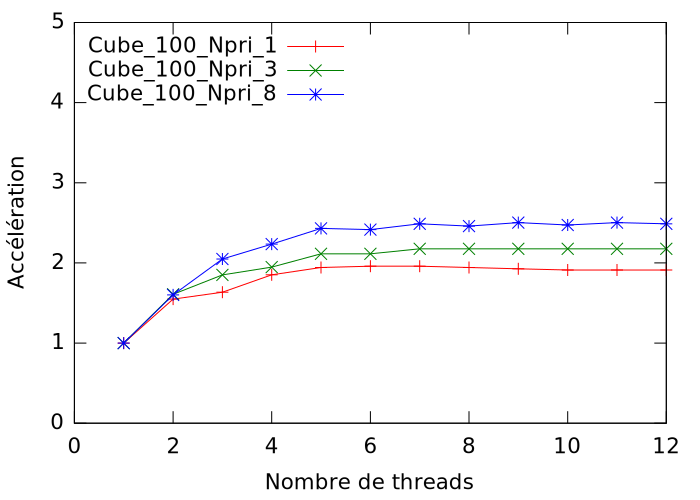
\includegraphics[width=0.7\textwidth]{res_spmv_omp}
  \caption{Accélération du produit matrice vecteur creux sur Rostand en mémoire partagée.}
  \label{fig:res_spmv_omp_rostand}
\end{figure}

%   (-_-)   %
\begin{figure}[t!]
  \centering
  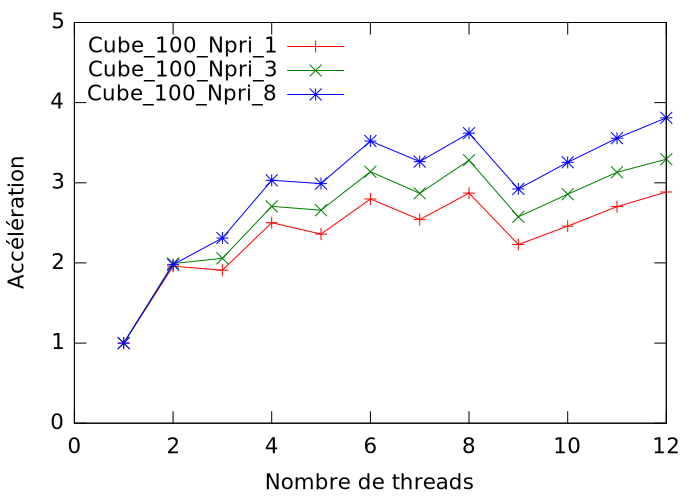
\includegraphics[width=0.7\textwidth]{res_spmv_mpi}
  \caption{Accélération du produit matrice vecteur creux sur Rostand en mémoire distribuée.}
  \label{fig:res_spmv_mpi_rostand}
\end{figure}




Sur la machine Manumanu, ces effets sont amplifiés (Fig.~\ref{fig:res_spmv_omp_manumanu}).
%
Nous obtenons les meilleurs performances en utilisant 8 coeurs avec une accélération de 5-6.
%
Utiliser plus de 8 coeurs pour effectuer le SpMV fait perdre du temps,
%
Les résultats en mémoire distribuée sont différents, les accélérations obtenues sont bien supérieures.
%
Les processus MPI sont alloués en mode compact, c'est à dire qu'ils sont distribués sur un minimum de noeud NUMA.
%
Avec 8 coeurs, nous retrouvons les même performances que la version en mémoire partagée (Fig.~\ref{fig:res_spmv_mpi_manumanu}).
%
Avec plus de processus, nous utilisons plus de noeud NUMA et nous obtenons une accélération maximal de 36.
%
En optimisant les accès mémoire de la version en mémoire partagée, nous pouvons donc espérer avoir ce même type d'accélération.


%   (-_-)   %
\begin{figure}[t!]
  \centering
  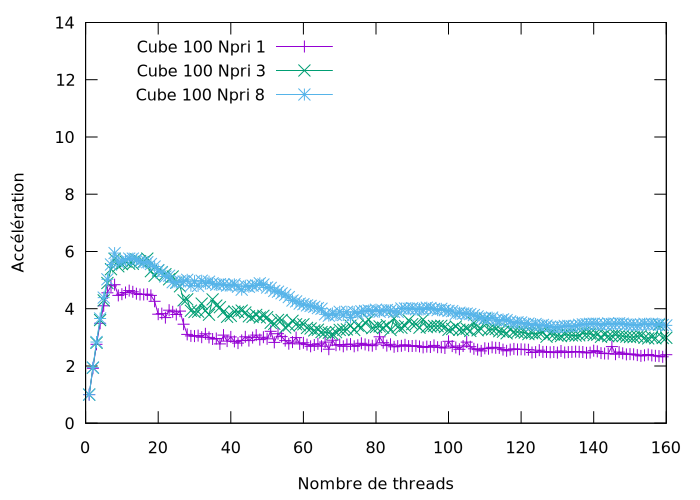
\includegraphics[width=0.7\textwidth]{res_spmv_omp_manu}
  \caption{Accélération du produit matrice vecteur creux sur Manumanu en mémoire partagée.}
  \label{fig:res_spmv_omp_manumanu}
\end{figure}

%   (-_-)   %
\begin{figure}[t!]
  \centering
  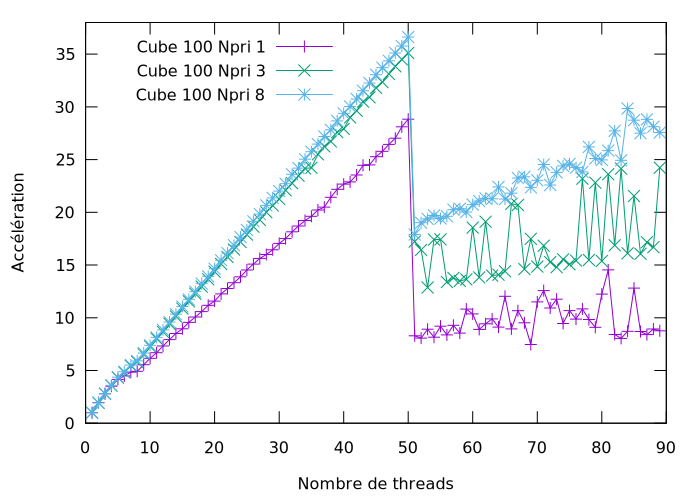
\includegraphics[width=0.7\textwidth]{res_spmv_mpi_manu}
  \caption{Accélération du produit matrice vecteur creux sur Manumanu en mémoire distribuée.}
  \label{fig:res_spmv_mpi_manumanu}
\end{figure}
